\RequirePackage[l2tabu, orthodox]{nag}
\RequirePackage{ifxetex}
\RequireXeTeX

\documentclass[tikz]{standalone}

%颜色
\usepackage{xcolor}

%长度
\usepackage{printlen}
\uselengthunit{mm}

%图形
\usepackage{pifont}
\usepackage{ean13isbn}
\usepackage{qrcode}
\usepackage{pdfpages}
\usepackage{overpic}
\usepackage{graphicx}

\usepackage{pstricks}

\usepackage{pgfplots}
\pgfplotsset{compat=1.16}
\usepackage{pgfmath}
\usepackage{pgf-pie}
\usetikzlibrary{calc}
\usetikzlibrary{shapes.geometric}
\usetikzlibrary{patterns}
\usetikzlibrary{arrows}
\usetikzlibrary{shapes}
\usetikzlibrary{chains}
\usetikzlibrary{mindmap}
\usetikzlibrary{graphs}
\usetikzlibrary{decorations.text}
\usetikzlibrary{arrows.meta}
\usetikzlibrary{shadows.blur}
\usetikzlibrary{shadings}

\usepackage{scsnowman}
\usepackage{circuitikz}
\usepackage{tikzpeople}
\usepackage{tikzducks}
\usepackage{flowchart}
\usepackage{smartdiagram}
\usepackage[edges]{forest}

%公式
\usepackage{amsmath}
\usepackage{amsthm}
\usepackage{amsfonts}
\usepackage{amssymb}
\usepackage{amsbsy}
\usepackage{amsopn}
\usepackage{amstext}
\usepackage{mathrsfs}
\usepackage{bm}
\usepackage{textcomp}
\usepackage{latexsym}
\usepackage{exscale}
\usepackage{relsize}
%\usepackage{xymtex}
\usepackage{physics}
\usepackage{siunitx}
\usepackage{hologo}
\usepackage{cases}

%文字
\usepackage{csquotes}
\usepackage{microtype}
\usepackage{ctex}

\csname
endofdump
\endcsname

\begin{document}

\begin{tikzpicture}[scale=1, transform shape]
	\tikzset{node distance=1.5cm}
	\node[anchor=south west,inner sep=0] (image) at (0,0) {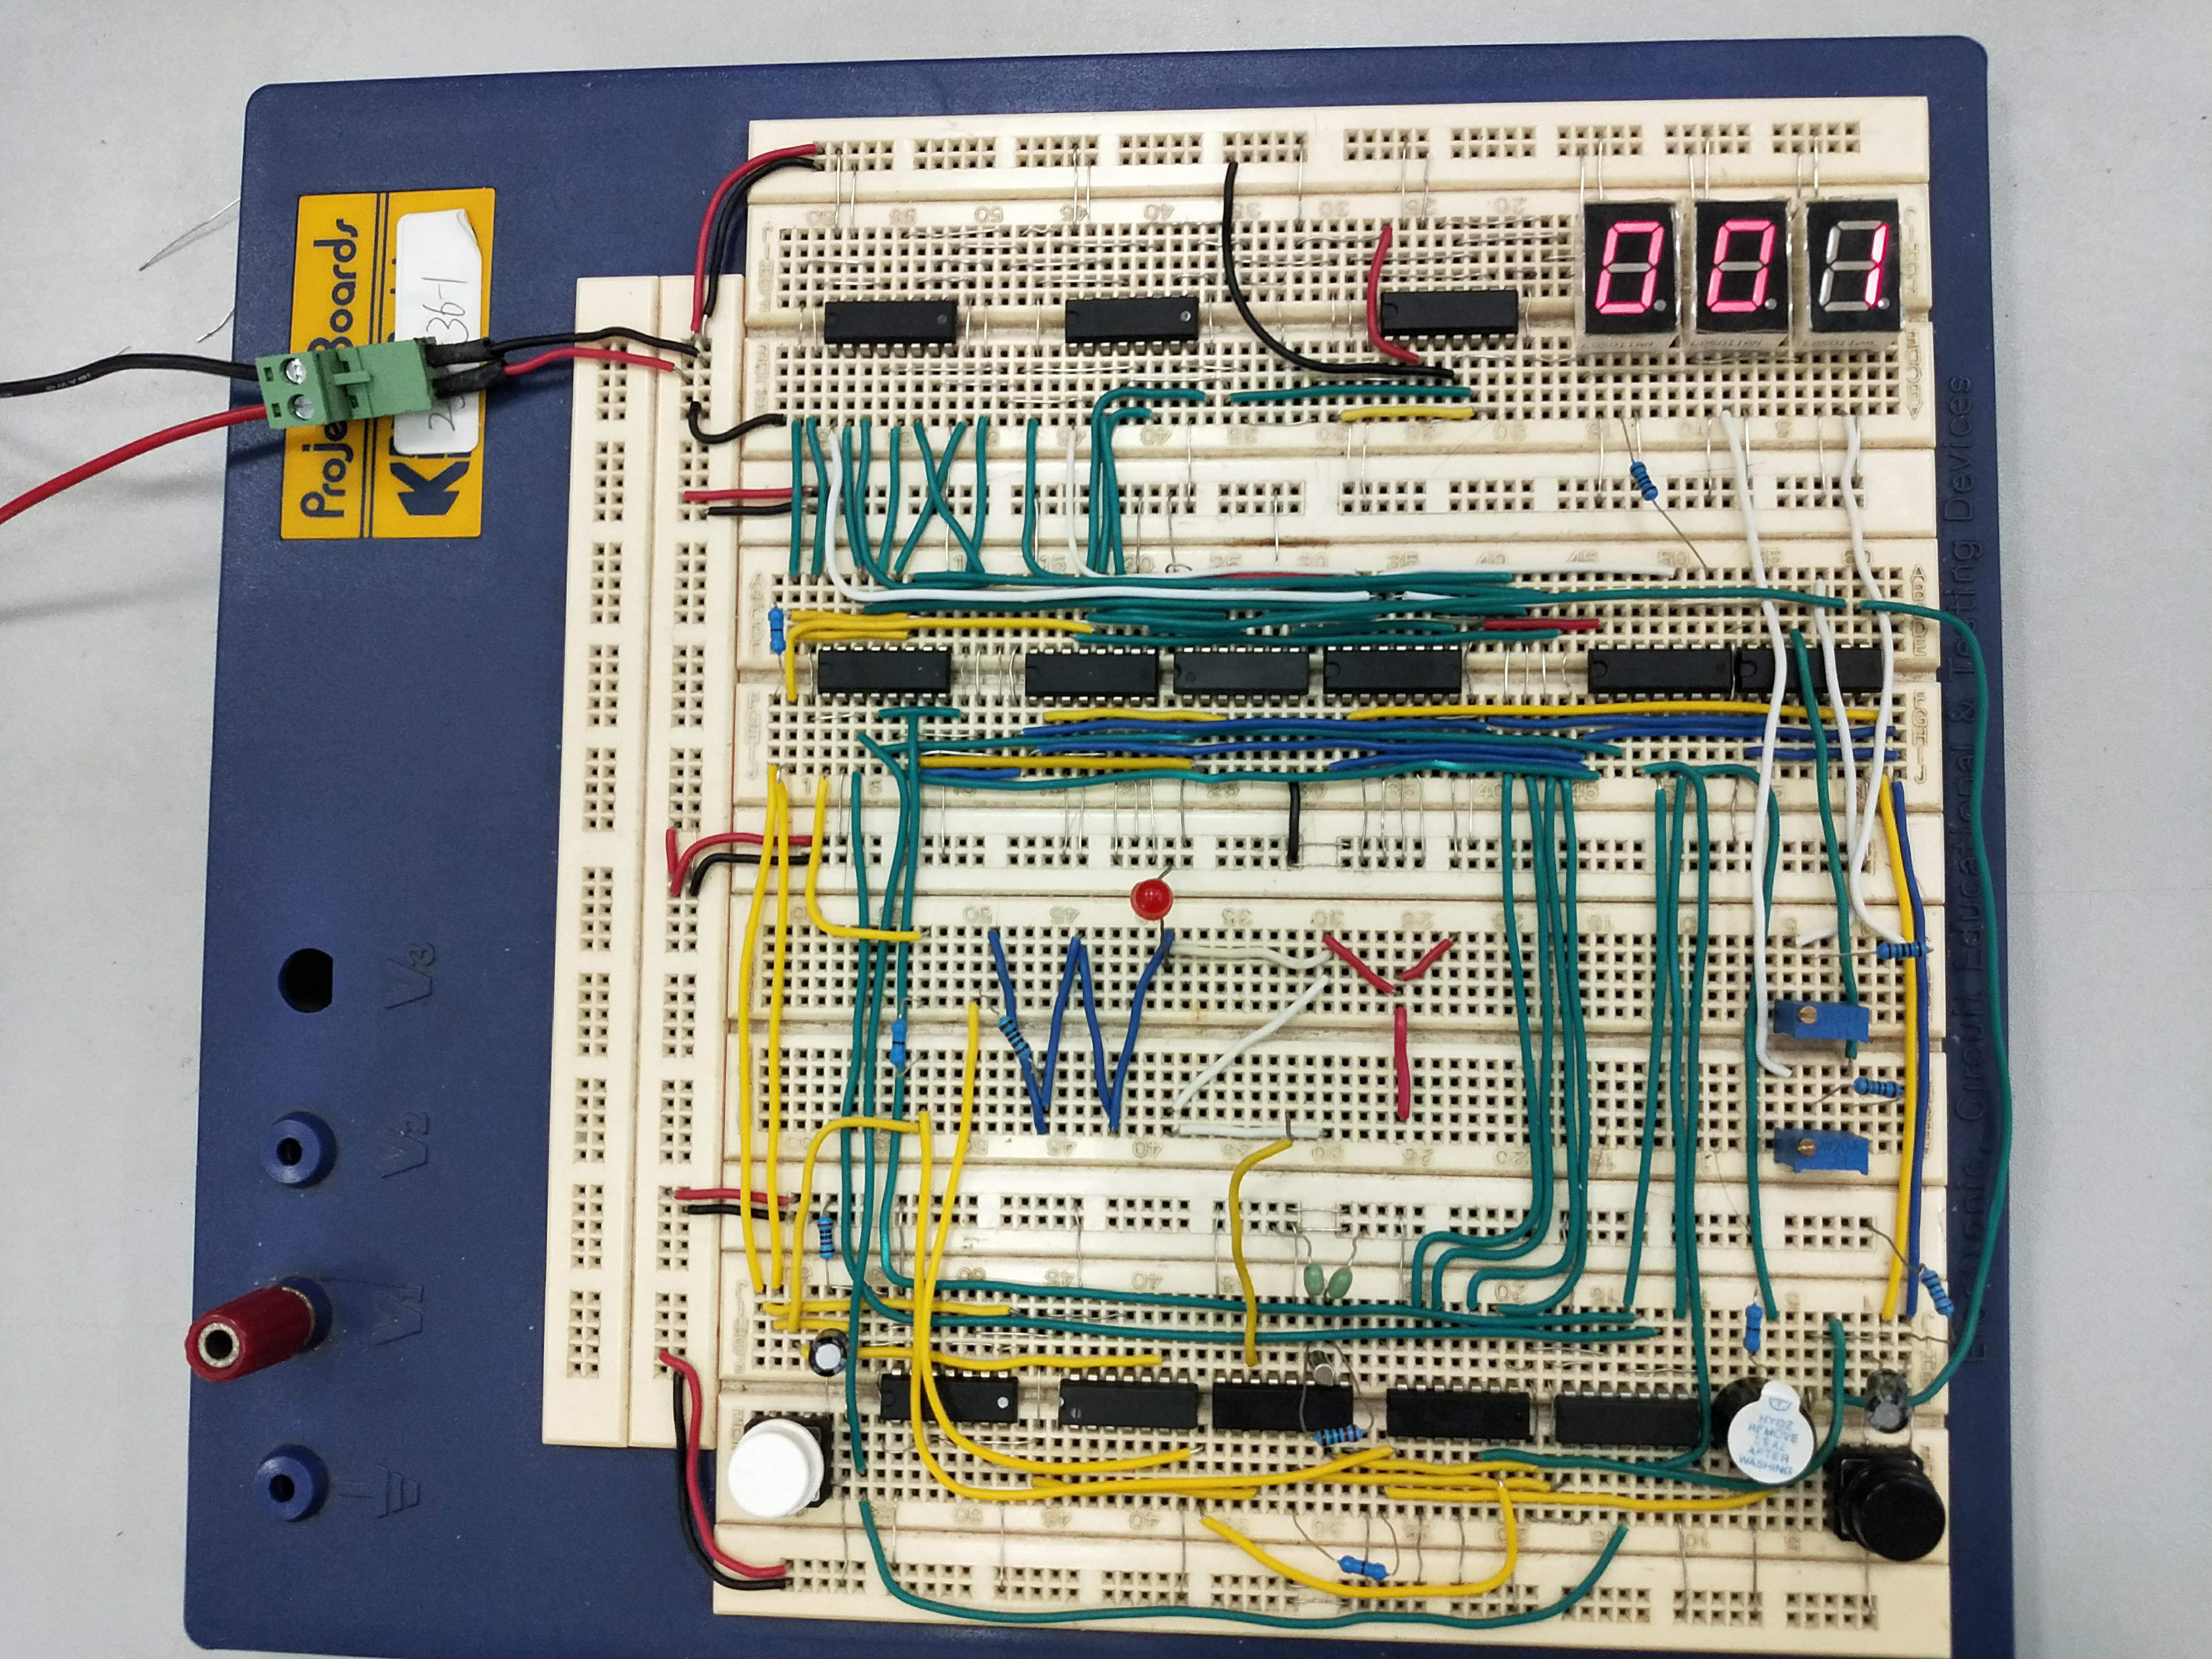
\includegraphics[width=0.9\textwidth]{bread0.png}};

	\begin{scope}[x={(image.south east)},y={(image.north west)}]

		%\draw[help lines,xstep=.1,ystep=.1] (0,0) grid (1,1);
		%\foreach \x in {0,1,...,9} {
		%\node [anchor=north] at (\x/10,0) {0.\x};
		%}
		%\foreach \y in {0,1,...,9} {
		%\node [anchor=east] at (0,\y/10) {0.\y};
		%}

		\draw[red, rounded corners] (.1,.7) rectangle (.25,.8);
		\node(电源总开关) at (.2,.8) [red, align=center, anchor=south] {\tiny 电源总开关};
		\draw[red, rounded corners] (.35,.75) rectangle (.7,.9);
		\node(动态译码) at (.55,.9) [red, align=center, anchor=south] {\tiny 动态译码};
		\draw[red, rounded corners] (.71,.75) rectangle (.86,.9);
		\node(显示) at (.8,.9) [red, align=center, anchor=south] {\tiny 显示};
		\draw[red, rounded corners] (.8,.29) rectangle (.88,.45);
		\node(亮度调节) at (.84,.45) [red, align=center, anchor=south] {\tiny 亮度调节};
		\draw[red, rounded corners] (.35,.55) rectangle (.55,.65);
		\node(计数) at (.45,.65) [red, align=center, anchor=south] {\tiny 计数};
		\draw[red, rounded corners] (.56,.55) rectangle (.88,.65);
		\node(动态选通) at (.75,.65) [red, align=center, anchor=south] {\tiny 动态选通};
		\draw[red, rounded corners] (.32,.08) rectangle (.47,.28);
		\node(校分) at (.4,.28) [red, align=center, anchor=south] {\tiny 校分};
		\draw[red, rounded corners] (.45,.3) rectangle (.68,.5);
		\node(信号指示) at (.55,.5) [red, align=center, anchor=south] {\tiny 信号指示};
		\draw[red, rounded corners] (.48,.1) rectangle (.62,.22);
		\node(脉冲发生) at (.55,.22) [red, align=center, anchor=south] {\tiny 脉冲发生};
		\draw[red, rounded corners] (.63,.1) rectangle (.82,.22);
		\node(报时) at (.72,.22) [red, align=center, anchor=south] {\tiny 报时};
		\draw[red, rounded corners] (.83,.05) rectangle (.9,.24);
		\node(清零) at (.86,.24) [red, align=center, anchor=south] {\tiny 清零};
	\end{scope}
\end{tikzpicture}

\end{document}

